\documentclass{letter}
\usepackage{graphicx}

\begin{document}

Nous avons test\'e la k-coloration avec 3 graphes assez proches. Le premier
graph est 2-coloriable. Le second est 3-coloriable et le dernier 4-coloriable.
Nous avons v\'erifi\'e qu'un graph 3-coloriable est bien 4-coloriable et pas
2-coloriable.

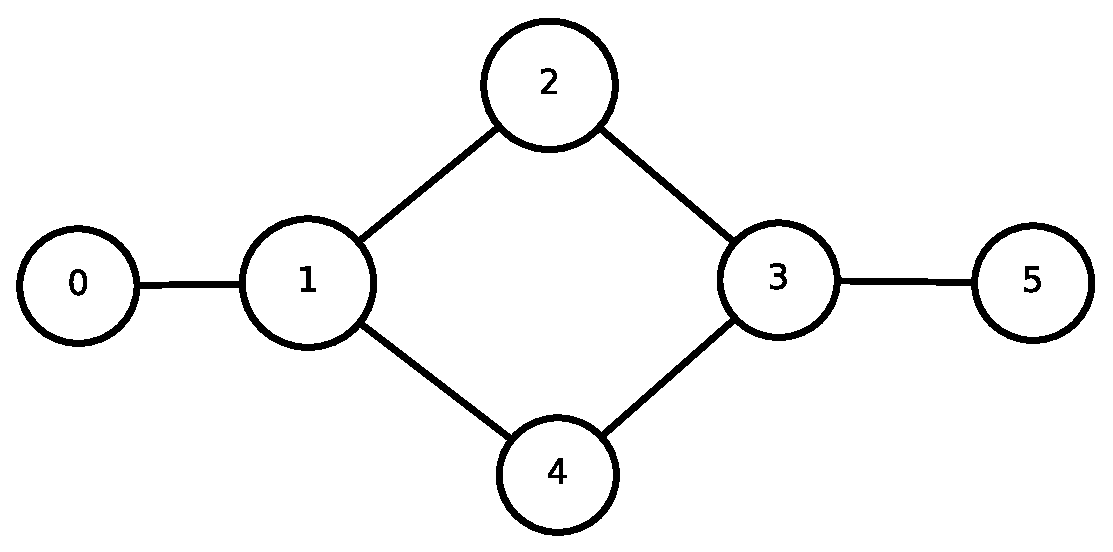
\includegraphics[scale=0.3]{test-2-color.eps}
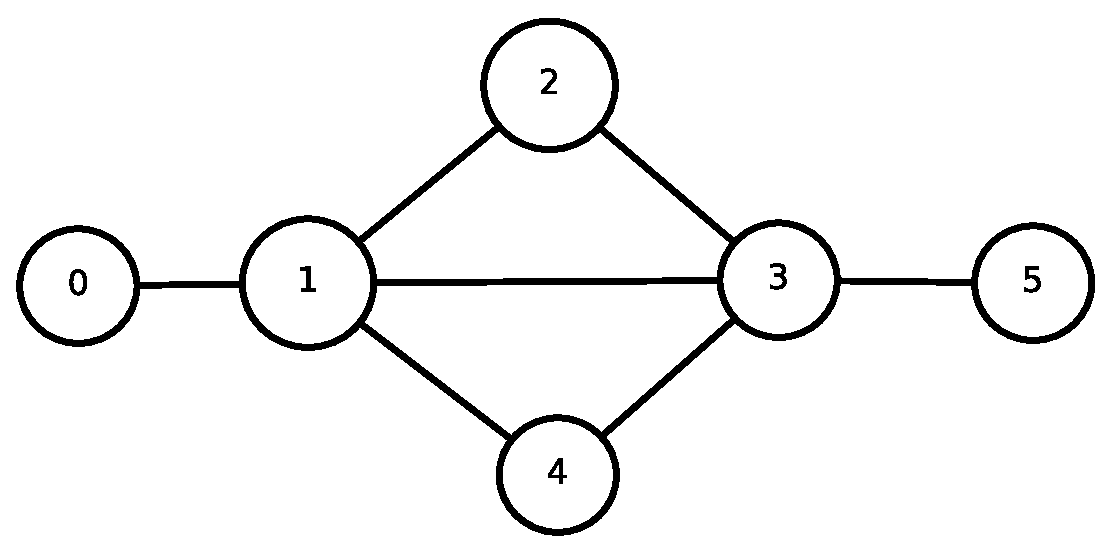
\includegraphics[scale=0.3]{test-3-color.eps}

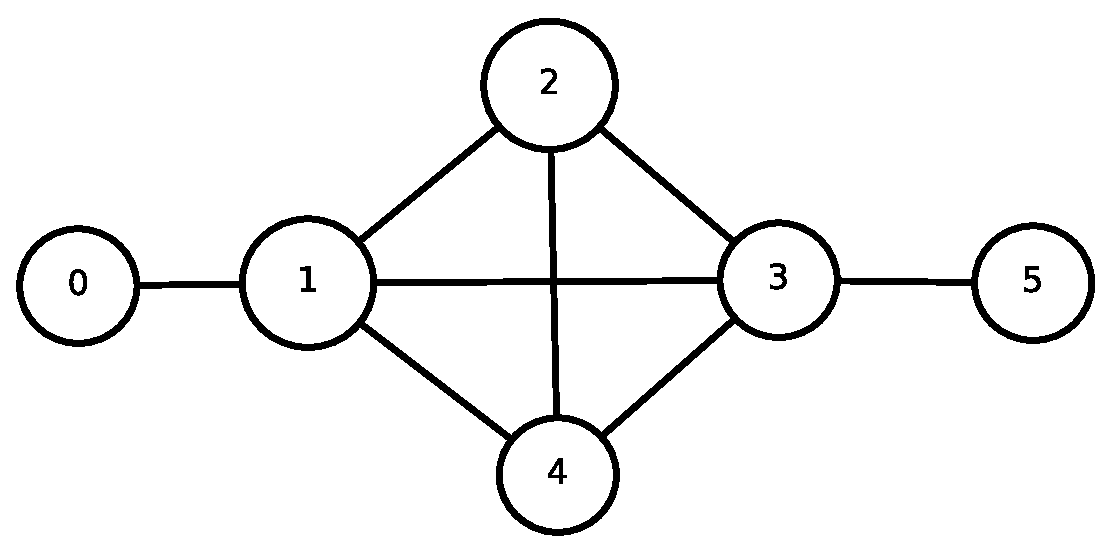
\includegraphics[scale=0.3]{test-4-color.eps}

Nous avons test\'e le chemin et le circuit hamiltonien. Nous avons cr\'e\'e deux graphes
assez proche des pr\'ec\'edents. Le premier a un chemin hamiltonien et le second un circuit 
hamiltonien.

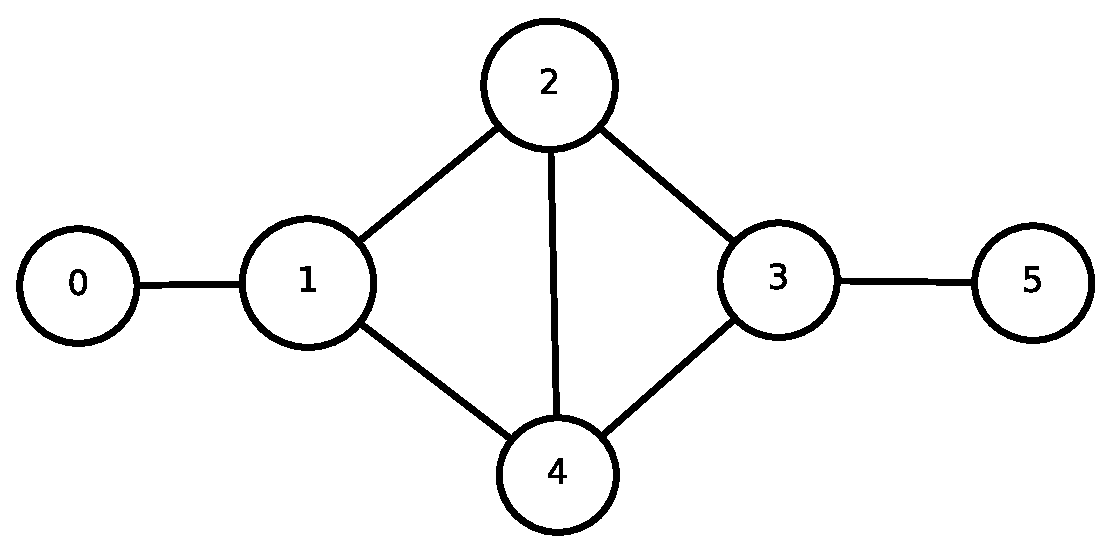
\includegraphics[scale=0.3]{test-hamiltonian-path.eps}
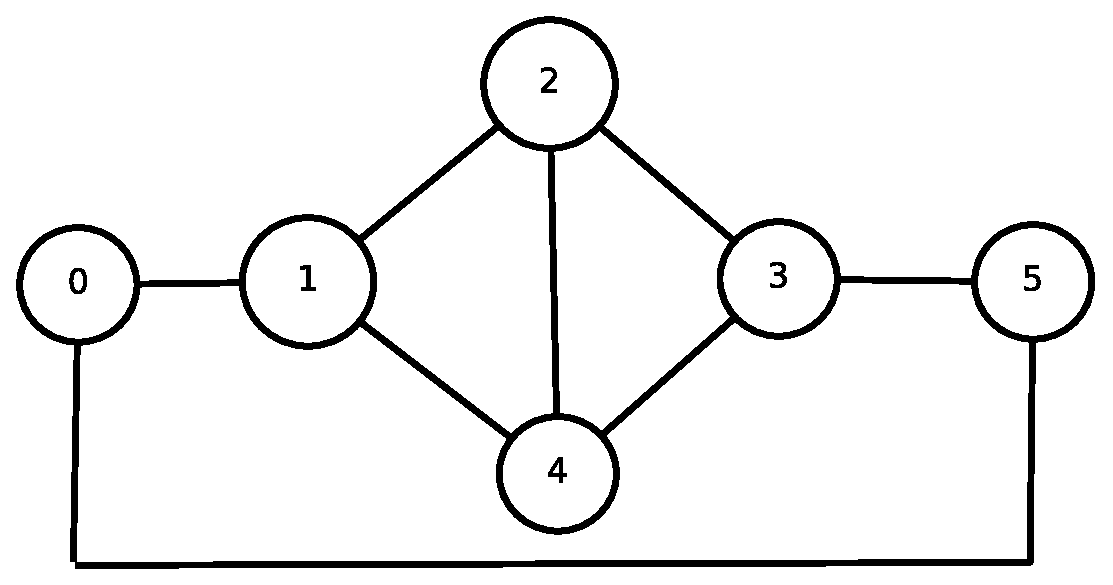
\includegraphics[scale=0.3]{test-hamiltonian-circuit.eps}

Nous avons test\'e que le circuit et le chemin soient bien d\'etect\'e, ainsi
qu'il n'y a pas de chemin avec le graphe qui a seulement un chemin, et finalement 
qu'il n'y a pas de chemin dans le graphe 2-coloriable.

Pour tester la clique nous avons cr\'e\'e un graphe qui a deux cliques, une de taille 3
et une autre de taille 4. 

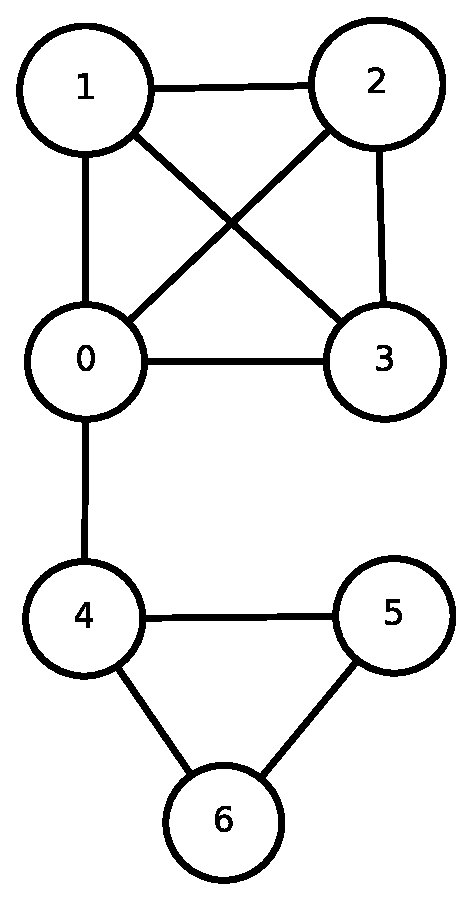
\includegraphics[scale=0.3]{test-clique.eps}

Nous avons v�rifi\'e que quand on demande une clique de taille 3 le r�sultat est bien les sommets 4,5 et 6
et que quand on demande une clique de taille 4 on a bien 0,1,2 et 3.

Pour la couverture de sommet, nous avons cr\'e\'e un graphe et son inverse.

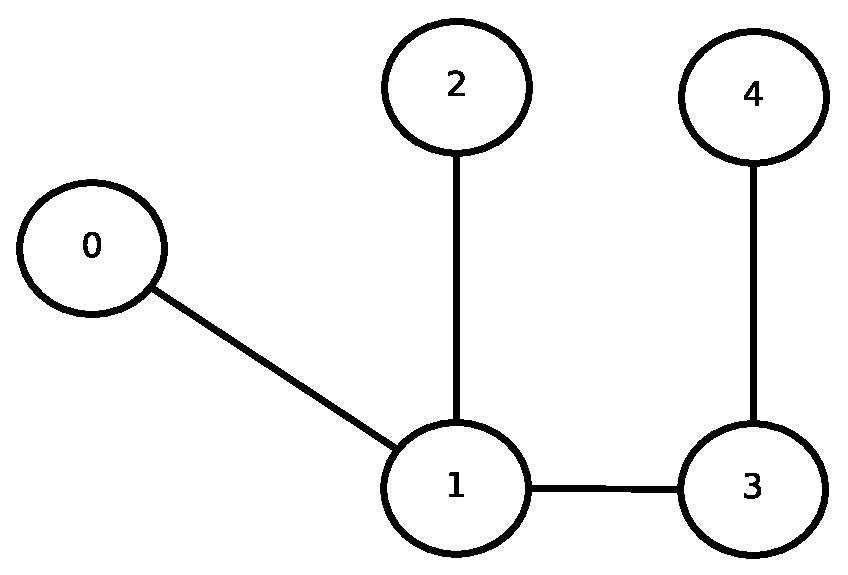
\includegraphics[scale=0.3]{test-vertex-cover.eps}
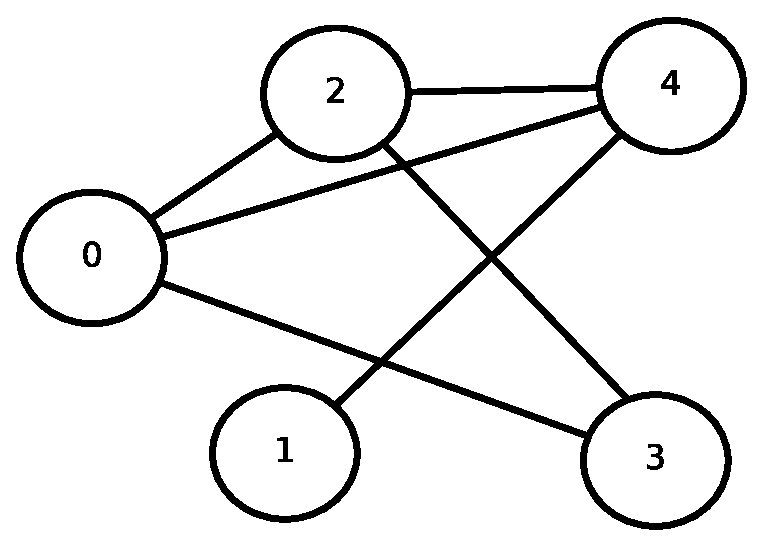
\includegraphics[scale=0.3]{test-vertex-cover-inv.eps}

On v�rifie donc que l'on a bien un couverture de sommet de taille 2 dans le graphe et une clique de taille 3 
dans son inverse contenant les sommets qui ne sont pas dans la couverture du premier.

Pour tester l'ensemble ind�pendant, nous avons utilis� les deux pr\'ec\'edents, en v�rifiant qu'une clique sur l'un
est bien un ensemble ind�pendant sur l'autre

\end{document}
